\documentclass{bredelebeamer}

%%%%%%%%%%%%%%%%%%%%%%%%%%%%%%%%%%%%%%%%%%%%%%%%

\title[Programación en MatLAB]{Introducción a la programación con MatLAB}
\subtitle{Módulo 09 - Funciones lógicas y estructuras de control}

\author{Autor1 - Autor2 - Autor3\inst{1}}
\institute[UTN.BA]
{
  \inst{1}%
  Universidad Tecnológica Nacional\\
  Facultad Regional Buenos Aires
  }

\date{dia mes 2018}

\subject{Taller de programación}

\logo{

\includegraphics[scale=0.15]{images/logo.png}
}

%%%%%%%%%%%%%%%%%%%%%%%%%%%%%%%%%%%%%%%%%%%%%%%%%%%%%%%%%%%%%%%%%%%%%
\begin{document}

\begin{frame}
  \titlepage 
\end{frame}

%%%%%%%%%%%%%%%%%%%%%%%%%%%%%%%%%%%%%%%%%%%%%%%%%%%%%%%%%%%%%%%%%%%%%

% Funciones lógicas y estructuras de control

%%%%%%%%%%%%%%%%%%%%%%%%%%%%%%%%%%%%%%%%%%%%%%%%%%%%%%%%%%%%%%%%%%%%%
\section{Funciones lógicas y estructuras de control}

\begin{frame}{Introducción}
Las secciones de código de los programas se pueden categorizar en una de tres estructuras:\\
\begin{itemize}
\item Secuencias: Lista de comandos que se ejecutan una a continuación de la otra.
\item Estructura de selección: Permite ejecutarse un comando si algún criterio es verdadero y otro si el criterio es falso.
\item Estructura de repetición: Hace que un grupo de comandos se ejecute varias veces.
\end{itemize}
\begin{block}{Tener en cuenta}
Las estructuras de selección y repetición dependen de operadores relacionales y lógicos.
\end{block}
\end{frame}

\begin{frame}{Introducción}
\begin{center}
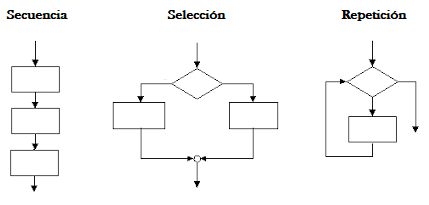
\includegraphics[scale=0.7]{images/pantalla3.png}
\end{center}
\end{frame}

\begin{frame}{Operadores relacionales}
Matlab tiene seis operadores relacionales para comparar dos matrices de igual tamaño. Los mismos son:\\
\begin{table}[]
\centering
\begin{tabular}{|c|c|}
\hline
Operador relacional & Interpretación      \\ \hline
\textless{}         & Menor que           \\ \hline
\textless{}=        & Menor que o igual a \\ \hline
\textgreater{}      & Mayor que           \\ \hline
\textgreater{}=     & Mayor que o igual a \\ \hline
==                  & Igual a             \\ \hline
$\sim$=             & no igual a          \\ \hline
\end{tabular}
\end{table}
Las comparaciones pueden ser verdaderas ó falsas. Matlab toma un valor positivo como verdadero(true) o cero como falso(false).
\end{frame}

\begin{frame}{Operadores relacionales}
Ej. Ejecutar las siguientes líneas. Obtener conclusiones.
\boiteviolette{
x = 5;\\
y = 1;\\
x<y;
}
Ej. Ejecutar las siguientes líneas. Obtener conclusiones.
\boiteviolette{
x = 1:5;\\
y = x-4;\\
x<y;
}
\end{frame}

\begin{frame}{Operadores relacionales}
Ej. Ejecutar las siguientes líneas. Obtener conclusiones.
\boiteviolette{
x = [1 2 3 4 5];\\
y = [-2 0 2 4 6];\\
x<y;
}
\begin{alertblock}{Tener en cuenta}
Para que una comparación sea verdadera, debe ser \textbf{verdadera} para cada elemento de la matriz.
\end{alertblock}
\end{frame}

\begin{frame}{Operadores lógicos}
Matlab permite combinar comparaciones mediante los operadores lógicos. Los mismos son:
\begin{table}[]
\centering
\begin{tabular}{|c|c|}
\hline
operador lógico & Interpretación \\ \hline
\&              & and            \\ \hline
$\sim$          & not            \\ \hline
|               & or             \\ \hline
\end{tabular}
\end{table}
\end{frame}

\begin{frame}{Operadores lógicos}
Ej. Ejecutar las siguientes líneas. Obtener conclusiones.
\boiteviolette{
x = [1 2 3 4 5];\\
y = [-2 0 2 4 6];\\
z = [8 8 8 8 8];\\
(z>x)\&(z>y);
}
Cómo leemos \textbf{(z>x)\&(z>y)} ?
\end{frame}

\begin{frame}{Estructura de selección - if}
\begin{columns}
\begin{column}{0.5\textwidth}
\begin{center}
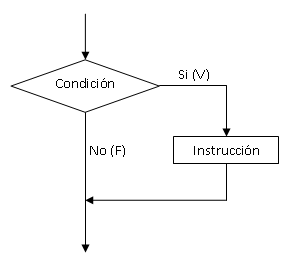
\includegraphics[scale=0.5]{images/pantalla5.png}
\end{center}
\end{column}
\begin{column}{0.3\textwidth}
if \textit{enunciado de comparación}\\
	....\\
    instrucciones\\
end
\end{column}
\end{columns}
\begin{center}
En este caso se ejecutan los comandos si y sólo si la condición es verdadera
\end{center}
\end{frame}

\begin{frame}{Estructura de selección - if/else}
\begin{columns}
\begin{column}{0.5\textwidth}
\begin{center}
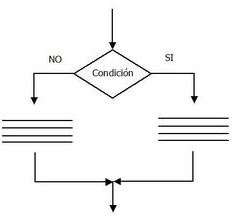
\includegraphics[scale=0.5]{images/pantalla4.png}
\end{center}
\end{column}
\begin{column}{0.3\textwidth}
if \textit{enunciado de comparación}\\
	....\\
    instrucciones 1\\
else\\
 	....\\
    instrucciones 2\\
end
\end{column}
\end{columns}
\begin{center}
En este caso se ejecutan las instrucciones 1 si la condición es verdadera y las instrucciones 2 si la condición es falsa. 
\end{center}
\end{frame}

\begin{frame}{Estructura de selección - elseif}
\begin{columns}
\begin{column}{0.5\textwidth}
\begin{center}
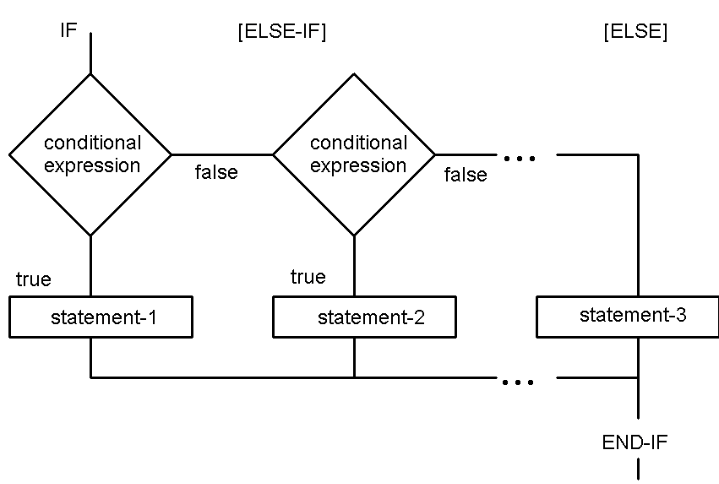
\includegraphics[scale=0.2]{images/pantalla6.png}
\end{center}
\end{column}
\begin{column}{0.3\textwidth}
if \textit{enunciado de comparación}\\
	....\\
    instrucciones 1\\
elseif \textit{enunciado de comparación}\\
 	....\\
    instrucciones 2\\
elseif \textit{enunciado de comparación}\\
 	....\\
    instrucciones 3\\
else\\
 	....\\
    instrucciones 4\\
end
\end{column}
\end{columns}
Se ejecutan las instrucciones 1 si condición 1 es cierta, se ejecutan las instrucciones 2 si condición 1 es falsa y condición 2 es cierta, continua sucesivamente. En caso de que todas sean falsas ejecuta las instrucciones 4.
\end{frame}

\begin{frame}{Ejercicio práctico xx}
Escriba una función if para cada uno de los siguientes problemas si supone que la entrada a la función es un escalar.
\begin{enumerate}
\item Suponga que en un estado la edad legal para beber es 21. Escriba y pruebe una función para determinar si una persona es lo suficientemente madura para beber.
\item Cuando una parte se fabrica, las dimensiones usualmente se especifican con una tolerancia. Suponga que cierta parte necesita tener 5.4cm de largo, más o menos 0.1cm (5.4 +/- 10cm). Escriba una función para determinar si una parte está dentro de dichas especificaciones.
\end{enumerate}
\end{frame}

\begin{frame}{Estructura de selección - Switch/case}
La instrucción switch ejecuta ciertas sentencias basadas en el valor de una
variable o expresión. Su sintaxis es:
\begin{columns}
\begin{column}{0.5\textwidth}
\begin{center}
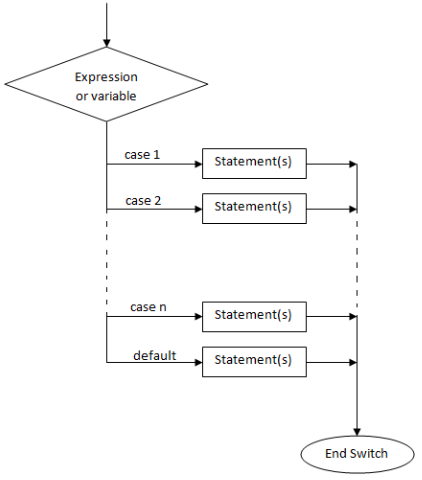
\includegraphics[scale=0.2]{images/pantalla7.png}
\end{center}
\end{column}
\begin{column}{0.5\textwidth}
switch \textit{expresión}\\
   case opcion 1\\
      instrucciones 1\\
   case opcion 2\\
      instrucciones 2\\
   otherwise
      instrucciones n\\
end
\end{column}
\end{columns}

\begin{block}{Tener en cuenta}
\textbf{Otherwise} no se requiere para que funcione la estructura switch/case.
\end{block}
\end{frame}

\begin{frame}{Menu}
\begin{exampleblock}{Comando}
Ver comando: \textbf{menu}
\end{exampleblock}
La función \textbf{menu} se usa en conjunto con una estructura switch/case.
Ej. Ejecutar las siguientes líneas. Obtener conclusiones.
\boiteviolette{
opcion = menu('Mi primer menu','opcion 1','opcion 2');\\
switch opcion\\
    case 1\\
        disp('opcion 1')\\
    case 2\\
        disp('opcion 2')\\
end
}
\end{frame}

\begin{frame}{Ejercicio práctico xx}
\begin{enumerate}
\item Cree un programa que pida al usuario su año en la escuela: primero, segundo, tercero o cuarto. La entrada sera una cadena. Use la estructura switch/case para determinar qué día serán los finales para cada grupo: lunes para primero, martes para segundo, miércoles para tercero y jueves para cuarto.
\item Repita el problema 1 pero esta vez con un menú
\item Cree un programa que pida al usuario ingresar el número de dulces que le gustaría comprar. La entrada será un número. Use la estructura switch/case para determinar la cuenta, donde:
\begin{itemize}
\item 1 dulce = 0.75\$
\item 2 dulces = 1.25\$
\item 3 dulces = 1.65\$
\end{itemize}
más de 3 dulces = 1.65\$ + 0.3 * (número ordenado -3)
\end{enumerate}
\end{frame}

\begin{frame}{Estructura de repetición - for}
\begin{columns}
\begin{column}{0.5\textwidth}
\begin{center}
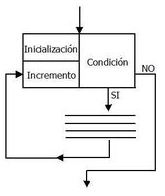
\includegraphics[scale=0.7]{images/pantalla8.png}
\end{center}
\end{column}
\begin{column}{0.3\textwidth}
for \textit{indice = comienzo\textbf{:}incremento\textbf{:}final}\\
   instrucciones\\
end
\end{column}
\end{columns}
\begin{center}
Las instrucciones dentro del bucle for se repiten N veces donde N es el valor final.
\end{center}
\end{frame}

\begin{frame}{Ejercicio práctico xx}
Considere la siguiente matriz de valores: x = [45,23,17,34,85,33] determine cuántos elementos son mayores que 30 utilizando un contador. \textit{Ayuda: Utilice la función length().}
\end{frame}

\begin{frame}{Estructura de repetición - while}
\begin{center}
Permite ejecutar de forma repetitiva un grupo de instrucciones mientras se cumpla una condición lógica especificada. La sintaxis es:
\end{center}
\begin{columns}
\begin{column}{0.5\textwidth}
\begin{center}
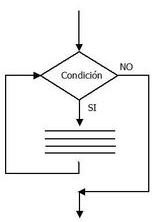
\includegraphics[scale=0.7]{images/pantalla9.png}
\end{center}
\end{column}
\begin{column}{0.3\textwidth}
while \textit{criterio}\\
   instrucciones\\
end
\end{column}
\end{columns}
\end{frame}

\begin{frame}{Ejercicio práctico xx}
Considere la siguiente matriz de valores: x = [45,23,17,34,85,33] determine cuántos elementos son mayores que 30 utilizando un contador. \textit{Ayuda: Utilice la función length().}
\end{frame}

\begin{frame}{Instrucción break y continue}
\begin{itemize}
\item La instrucción \textbf{break} finaliza la ejecución de un bucle for o while (de forma prematura). A continuación se ejecuta la siguiente instrucción fuera de dicho bloque.
\item La instrucción \textbf{continue} pasa el control a la iteración siguiente en un bucle for o while en el cual aparece ignorando las restantes instrucciones en el cuerpo del bucle.
\end{itemize}
\end{frame}

%%%%%%%%%%%%%%%%%%%%%%%%%%%%%%%%%%%%%%%%%%%%%%%%%%%%%%%%%%%%%%%%%%%%%

% Sección de consultas

%%%%%%%%%%%%%%%%%%%%%%%%%%%%%%%%%%%%%%%%%%%%%%%%%%%%%%%%%%%%%%%%%%%%%

\section{Consultas}
\begin{frame}{Consultas}
\begin{center}

\includegraphics[scale=0.3]{images/consultas.png}
\end{center}
\end{frame}


%%%%%%%%%%%%%%%%%%%%%%%%%%%%%%%%%%%%%%%%%%%%%%%%%%%%%%%%%%%%%%%%%%%%%

% Sección de bibliografía

%%%%%%%%%%%%%%%%%%%%%%%%%%%%%%%%%%%%%%%%%%%%%%%%%%%%%%%%%%%%%%%%%%%%%

\section{Bibliografia}

\begin{frame}{Bibliografía}
\begin{columns}
\begin{column}{0.5\textwidth}
\begin{center}

\includegraphics[scale=0.4]{images/biblio1.png}
\end{center}
\end{column}
\begin{column}{0.5\textwidth}
\begin{center}
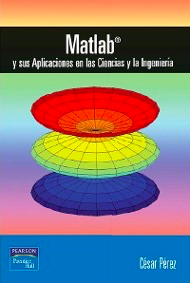
\includegraphics[scale=0.5]{images/biblio2.png}
\end{center}
\end{column}
\end{columns}
\end{frame}

\end{document}
